\section{Primacy of the first seconds}

Our main observations so far are: \one\ Vine micro videos appear to be different from both images (Flickr) and videos (YouTube) and \two\  content quality features, especially image-related ones (e.g., fraction of faces with frames) become  important for user engagement and popularity metrics. %and \three\ unlike videos where affect (sentiment) plays an important role in user engagement~\cite{bardzell2009understanding,fontanini2016web,eckler2011spreading}\footnote{See also {http://67.222.24.243/wp-content/uploads/2009/03/affect-study-screen-view.pdf} (accessed 24 Oct 2016).}, sentiments conveyed in the video appear to be much less important in Vine. 
In this section, we try to understand these findings further: One way to think about videos is as a sequence of images. With micro videos, this sequence is of course much shorter than in other videos. To see whether the visual content of micro videos is more image-like or video-like, we consider the impact and evolution of image-related features from the beginning to the end of the micro video. 

\subsection{Image quality deteriorates over time}




Vine videos can be at most 6.5 seconds long. We sample the videos twice every second and represent the whole video as a series of 12-13 static frames. This sampling rate is not too low to miss any considerable frame transitions, neither is it too high to include a lot of mid transition frames. For each sampled frame, we calculate the feature under consideration -- sentiment, percentage of faces, and aesthetic score. To compute the aesthetic score, we extract the 18 aesthetic features described in Table~\ref{tab:Features_table}. for each frame frame. To find an aggregate overall aesthetic score of each frame, we use a weighted sum of all the features (This is possible because all the features are on the same scale), where the weights are calculated to be proportional to the importance of each feature in the classifier designed in the previous section. 


For each video and each feature, we then compute when in the video the feature reached its maximum value. We then divide the videos into two second intervals, essentially dividing the video into its first third, second third and third third. We then ask what proportion of videos had the maximum value of a feature in the first (respectively second and third) third. This procedure tells us when we are likely to find the `best' part of the video. 

\begin{figure}[!htb]
\centering
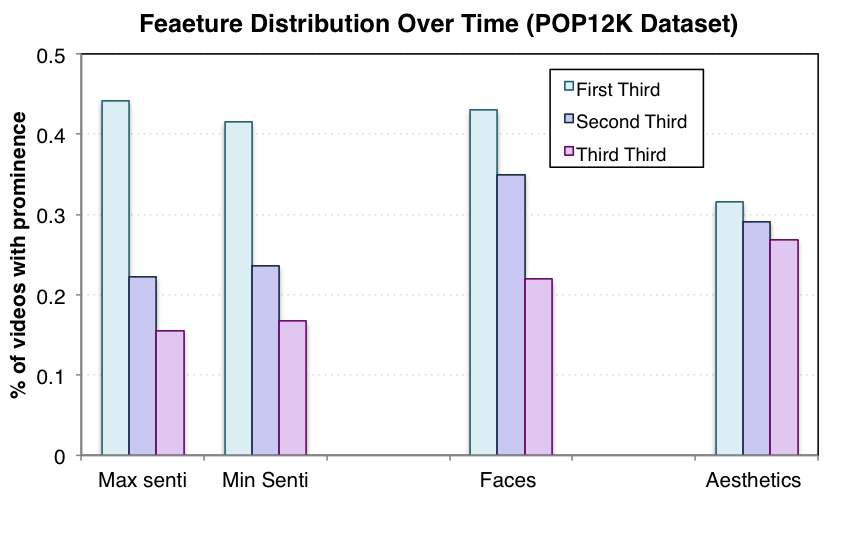
\includegraphics[width=\columnwidth]{plots/ThirdsDistribution.png}
\caption{\textsl{Evolution of Feature magnitude: The graph shows sharp trend in prevalence of strongest component of a feature in the first one third of the video. The strength decreases progressively for the successive thirds. (Results shown for POP12K dataset. Similar results obtained for ALL120K.)}}
\label{fig:Face_Thirds}
\end{figure}

Fig.~\ref{fig:Face_Thirds} shows the result for each major category of content-related feature, plotted over both our datasets (ALL120K and POP12K). We observe a general trend where the first third has the maximum (best) value for all features considered. For instance, the best aesthetic score is to be found in the first two seconds. Similarly, the proportion of faces, an important predictor of engagement (Fig.~\ref{fig:Face_CDF}), is also maximum in the first third. 

Note that for sentiment values, the minimum value is just as valid and valuable as the maximum, representing a sad or emotionally dark segment of the movie with negative sentiment, in contrast to a happy segment of the movie with positive sentiment. Therefore, we calculate which third of the movie we find the maximum and minimum sentiment values and plot these separately. In both cases, we find  yet again that the first third of the video has the maximum (minimum) sentiment value for the majority of videos. 

\subsection{Loops and likes are obtained on first sight: Initial seconds predict engagement}
\label{sec:first-seconds}
Collectively, the results above paint a picture where the first seconds of the micro video are highly important in engaging the user. We conjecture that this might be because of the mobile-first nature of Vine: the primary user interface is the Vine app, where users select which videos to watch by scrolling over it. The vine only plays when the user retains focus over the video, and hence the first seconds are likely critical for grabbing user attention and engaging them. 

We next take this result to its logical conclusion, and ask how the classifier developed in the previous section for predicting engagement would work if using only content-related features from the first third of the video rather than from the whole micro video. Following the same methodology as described in the previous sub-section, we develop a series of classifiers for different popularity thresholds, training this time on image content-related features drawn from the first two seconds of the video rather than from across the whole video. The same set of hyper parameters were used as in the previous setting. As shown in Fig.~\ref{fig:Classifier_performance}, the resulting classifiers (labeled 2 sec) perform very similarly to the classifiers developed before (labeled 6 sec). Further, Fig.~\ref{fig:Feature_importance} shows that the relative importance of different features is also nearly identical to the previous results. It should be emphasised that although these results were obtained using loop counts as the metric for user engagement, similar results have also been obtained using reposts (revines). 

These results point to a \emph{primacy of the first seconds} effect, whereby the first seconds of a micro video matter as much as the whole video, suggesting that they behave almost like still images in terms of user engagement.

%To validate and understand the significance of the primacy property, it was important to understand relation of engegement of users with the primal states of a micro video. Following the methodology of training iterative and progressively selective classifier, we set up an experiement where the classifier would be trained on features extracted only from the intial 2 seconds of vine mico video instead of the entire video. We chose aesthetic and sentiment features extracted from frames sampled in the first two seconds and repeated the classfier training with the same set of hyper parameters for the classifier. It can be observed from the \ref{fig:Classifier_performance}, that the classifier trained of the primal sections of the videos, resulted in identical or in some cases better results, when compared to the classifer trained on the whole video. This validates the hypotheis that producers are deliberately or inadvertantly creating contents that engage users in the first one third of the micro video. 






%In the previous Sections, we learnt that Vine can be seen as a new form of expression, lying in between the photographic and the video media. We further verify here this intuition by looking at how different features vary over time in a Vine video, thus gaining insights about the role of the temporal dimension in micro-videos.
%%To understand the phenomenon of user engagement with the micro-video content, 
%We extract the features listed in Sec. \ref{sec:features} from the video frames and the audio tracks.% The motivation behind this excercise was to find peculiar discriminators amongst these features with respect to engagement. 
%%The following section describes some of the saliant differences between the high engagement and low engagement micro videos. 
%We sample the videos twice every second and represent the whole 6-second long video as a series of 12 static frames. This sampling rate is not too low to miss any considerable frame transitions, neither is too high to include a lot of mid transition frames. We consider \textit{N} = 12,000 micro-videos,  6000 from POP12K and 6000 from ALL120K dataset. 
%
%\subsection{ Too short to make an impact ?}
%Image sentiment values computed using MVSO \cite{jou2015visual} detectors reflect the video sentiment as intended by its producer. %Because these detectors were trained on static images downloaded from Flickr they do a good job of understanding some sort of an abstract sentiment from an image. 
%We explore the time signatures generated by per-frame sentiment values over time.
%%of these abstract frame sentiments for micro-videos.  
%To do so, we use MVSO dectetors to compute the sentiment of each extracted frame on a scale of 1 to 5.% The detailed reasoning and description of this sentiment scale can be found in\cite{jou2015visual}. 
%We obtain a $\mathbf{M} = N \times 12$ matrix of sentiment time signatures. %for \textit{N} videos. I%n our case \textit{N} is 12,000 micro videos,
%To understand if there are any patterns in time-sentiment signatures across the videos,  we cluster the rows in the matrix $\mathbf{M}$  using K-means clustering algorithm. We vary the number of clusters K from one to 10 and use the \emph{elbow method} to choose the right K. %K-means is iteratively run over the complete dataset for different values of K ranging from 1 to a resonably high maximum. We run till K = 10. 
%The elbow method works by computing, for each K, the sum of squared distances $SSD_K$ between a cluster centroid and all the points that fall into that cluster:%. We therefore compute the SSD at each K:
%\begin{equation}
%SSD_K = \sum_{i =1}^{K} \sum_{X \in{N}}{dist(X,c_i)}^2
%\end{equation}
%The \emph{elbow}, i.e. the correct number of clusters, is the point in the plot of $SSD_K$ where a change in rate of decrease of SSDs occurs.
%We plot the SSD values (see Fig \ref{fig:Elbow_method}) and choose $K=4$.
%
%To look at  common sentiment trends in micro-videos, we plot the values of the centroids for each cluster in Fig \ref{fig:Clusters}. We notice that the 4 clusters are clearly separated in the sentiment space, but that, over time, sentiment values remain constant for a given cluster. This suggests that in general, no matter its polarity, sentiment in micro-videos remains constant for the whole duration. The paper does not explore the fundamental reason behind this, but it is a peculiar behaviour.  One possible reason behind this could be that a time-span of 6 seconds is too short to allow micro-video creators to project any kind of perceivable and impactful change in frame sentiments.  This it re-enforces our hypothesis of Vine being a medium in between images (no temporal dimension - constant sentiment) and long videos, whose stories contain changes in sentiment over time.

%\begin{figure}[!htb]
%\centering
%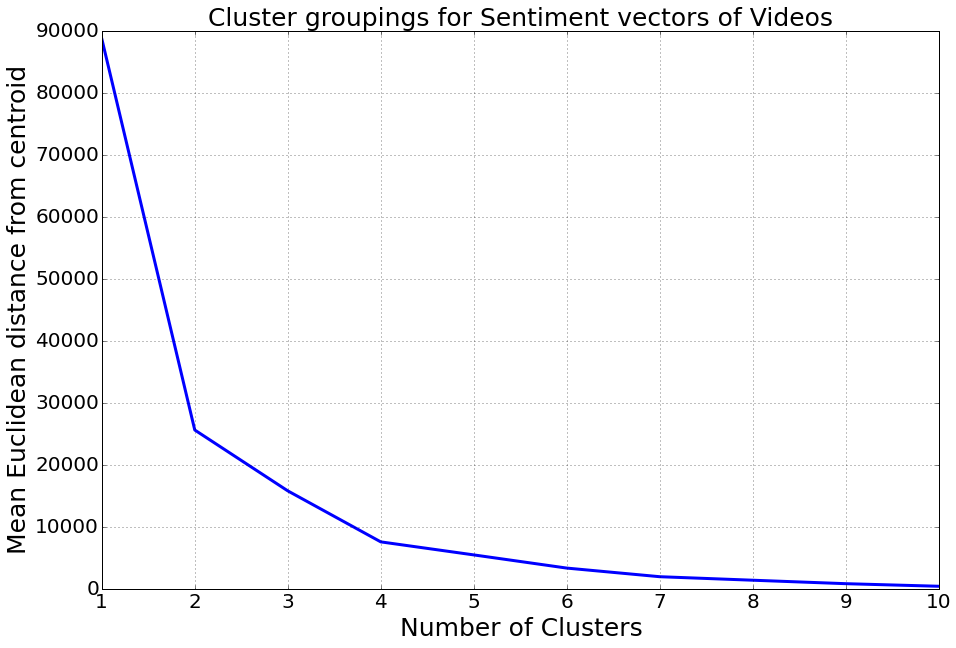
\includegraphics[width=\columnwidth]{plots/grouping_graph_clusters}
%\caption{\textsl{The Sentiment transition matrix was analysed for existence of clusters, using the elbow points method for mean Euclidean distance (Minkowski distance for p = 2). We found that the best grouping exists at K=4 }}
%\label{fig:Elbow_method}
%\end{figure}

%\begin{figure}[!htb]
%\centering
%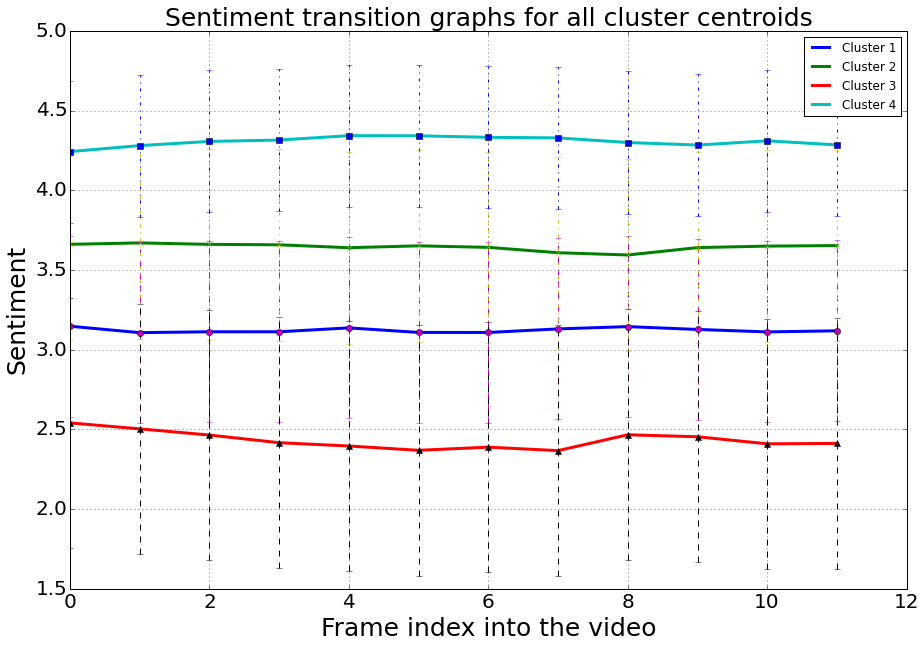
\includegraphics[width=\columnwidth]{plots/4_cluster_senti}
%\caption{\textsl{ Plot of frame sentiment vectors, of the 4 centroids of the clusters found. The vine videos  tend to have a constant sentiment structure at 4 distinct sentiment levels }}
%\label{fig:Clusters}
%\end{figure}

%\begin{figure}
%\centering
%\subfloat[\textsl{Plot of the sum of squared Euclidean distance for each cluster member from its centroid. The Elbow point exists at K=4 }]{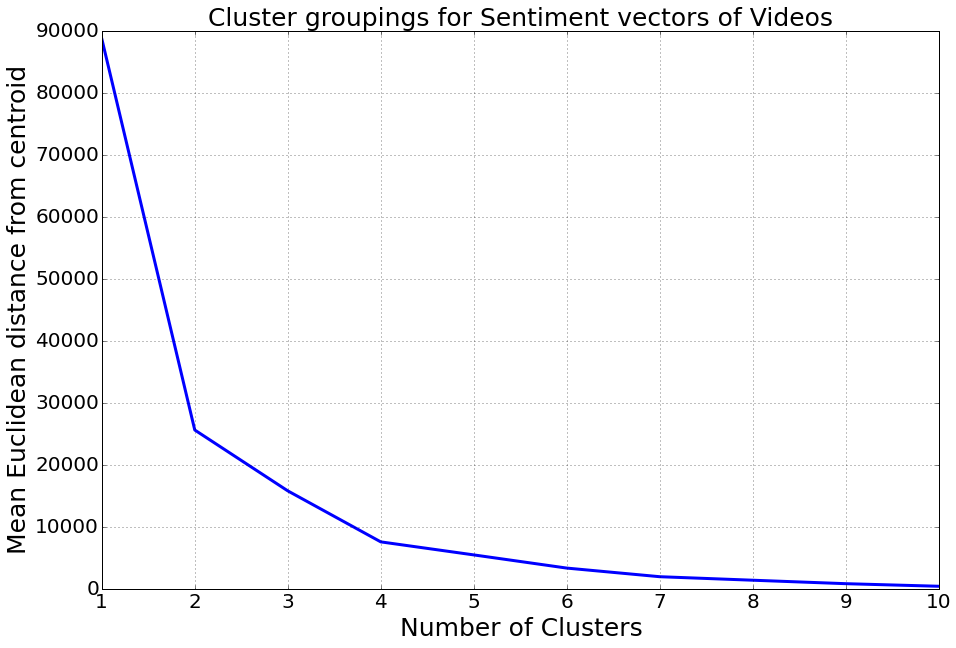
\includegraphics[width=0.5\columnwidth]{plots/grouping_graph_clusters}}
%\hfill
%\subfloat[\textsl{ Plot of frame sentiment vectors of the 4 centroids of the clusters found.}]{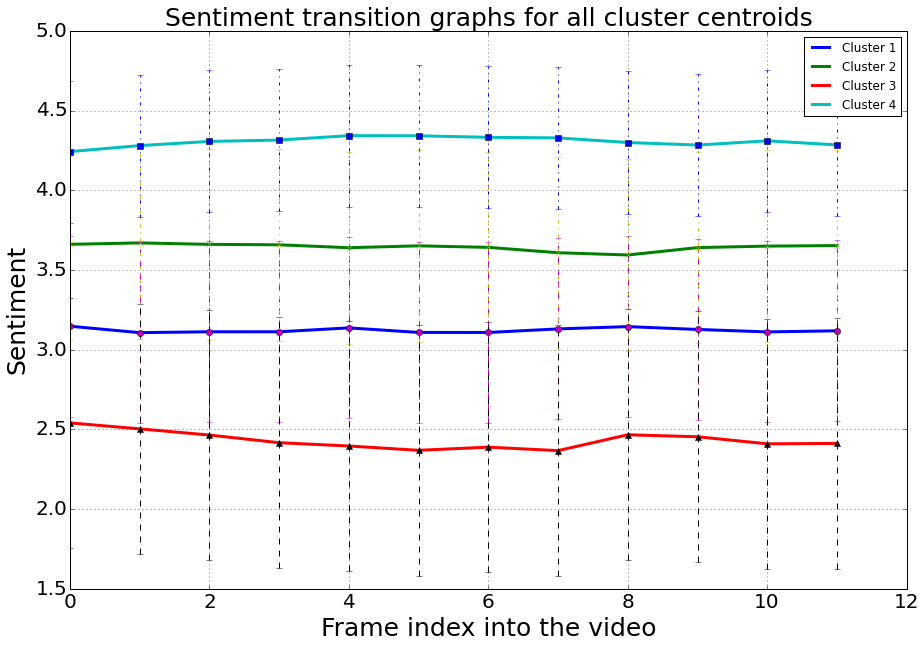
\includegraphics[width=0.5\columnwidth]{plots/4_cluster_senti}}
%\hfill\null
%\end{figure}

%\begin{figure*}[!htbp]
%\centering
%\hspace*{-5mm}
%\subfloat[Elbow point ]{
%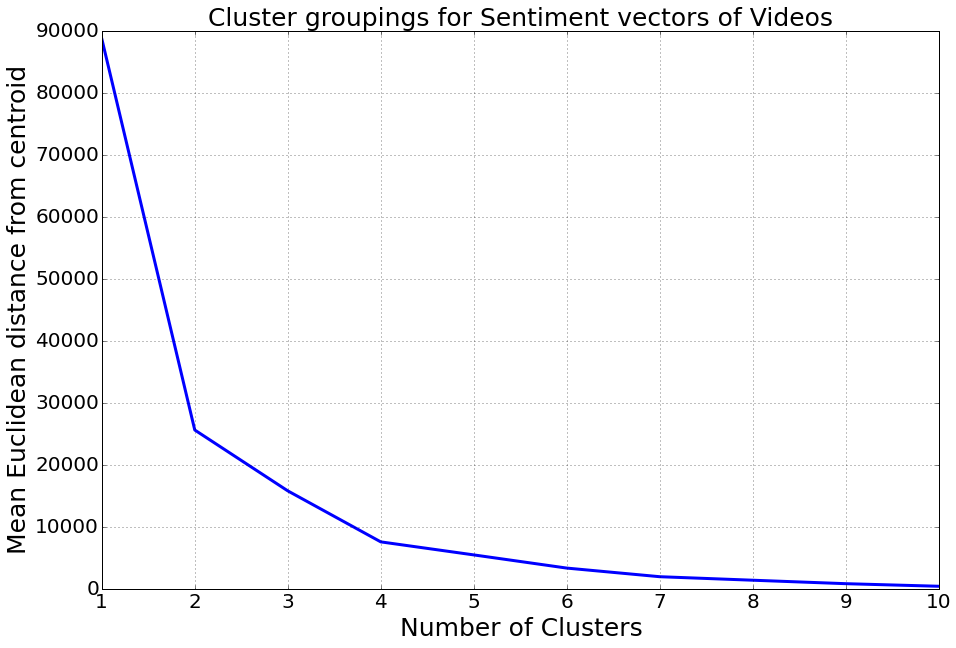
\includegraphics[width=0.40\textwidth]{plots/grouping_graph_clusters}
%\label{fig:Elbow_method}
%}
%\subfloat[Sentiment vectors of the 4 centroids ]{
%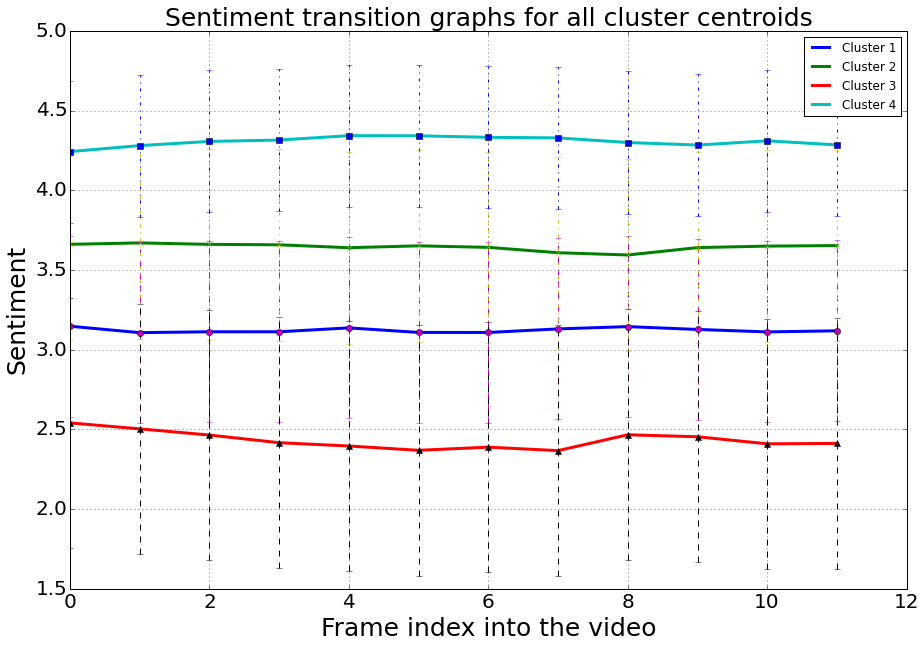
\includegraphics[width=0.40\textwidth]{plots/4_cluster_senti}
%\label{fig:Clusters}
%}
%\caption{(a) Plot of the Sum of squared Distances value for all the cluster ids. The elbow point is seen at K = 4 (b) Plot of frame sentiment vectors, of the 4 centroids of the clusters found. The vine videos  tend to have a constant sentiment structure at 4 distinct sentiment levels  }
%\end{figure*}



%\begin{figure}[!htb]
%\centering
%\includegraphics[width=\columnwidth]{plots/faceThirdsAnalysis}
%\caption{\textsl{The Plot represents the frequency of finding highest number of face frames in 1st , 2nd or 3rd onethirds of a micro video. This feature also shows a trend to be highest in the first one third of the video }}
%\label{fig:Face_Thirds}
%\end{figure}

%Using this elbow point, we cluster the Matrix and look for salient trends in transition, by plotting the values of centroids of each cluster. 


%\subsection{First impression lasts}
%Following this intuition, we made a second experiment. The whole idea of a user engaging with a micro video on Vine, involves the process of scrolling past videos and then keeping a video in focus so as to trigger the auto looping mechanism described in introduction. This whole user experience makes engagement highly influenced by how far the user plays the video. To understand the effect of frame sentiments in different parts if video over this user behaviour, we plotted a simple histogram of the frequency of occurrences of maximum or minimum frame sentiments against the thirds (i.e. intervals of 2 seconds) of a video. From Fig \ref{fig:Senti_Thirds}, an interesting trend emerges: the probability of coming across the most positive or the most negative sentiment in a micro video is  highest in the first one third of the video, and progressively decays.
%
%\begin{figure}[!htb]
%\centering
%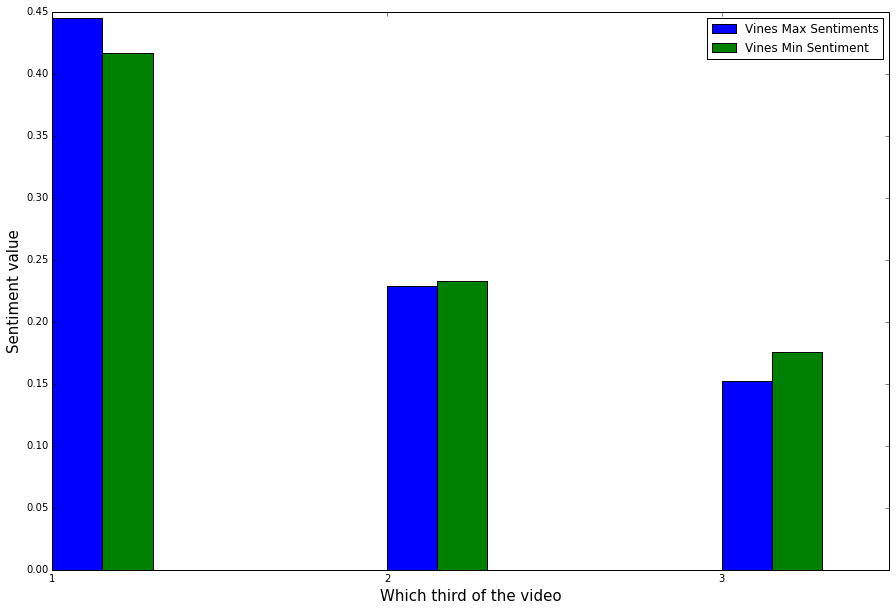
\includegraphics[width=\columnwidth]{plots/SentimentsThirds}
%\caption{\textsl{ Frequency of occurrence of maximum or minimum sentiment. For this graph, the video is considered in thirds, and the frequency of occurance of both max and min frame sentiments is plotted. }}
%\label{fig:Senti_Thirds}
%\end{figure} 

%\mr{Sagar can you explain more the following: how how do you know about the overall aesthetic quality?}\sj{Miriam- I will try to explain it, but the way I am aggregating is a very heuristic way of doing so. I need to find a better way to explain this. What I am doing is that I am taking a weighted sum of each of the 18 features evaluated per frame. The weights for these features are basically the feature importance values learnt from the classifier at the classifier's highest level of selectivity.}
%We repeated a similar process for aesthetic features. We compute the 18 aesthetic features for each frame frame. To find an aggregate overall aesthetic score of each frame, we use a weighted sum of all the features (This is possible because all the features are on the same scale). The weights were learnt from the classifier described in \ref{Designing a Classifier} when the classifier was trained to be highly selective in predicting popularity. These weights are basically proportional to the impact a particular aesthetic feature has over the popularity of the video according to the classifier. We found a similar trend of the first one third of video having the best overall aesthetic quality (Fig. \ref{fig:Aesthetic_trends}).

%\begin{figure}[!htb]
%\centering
%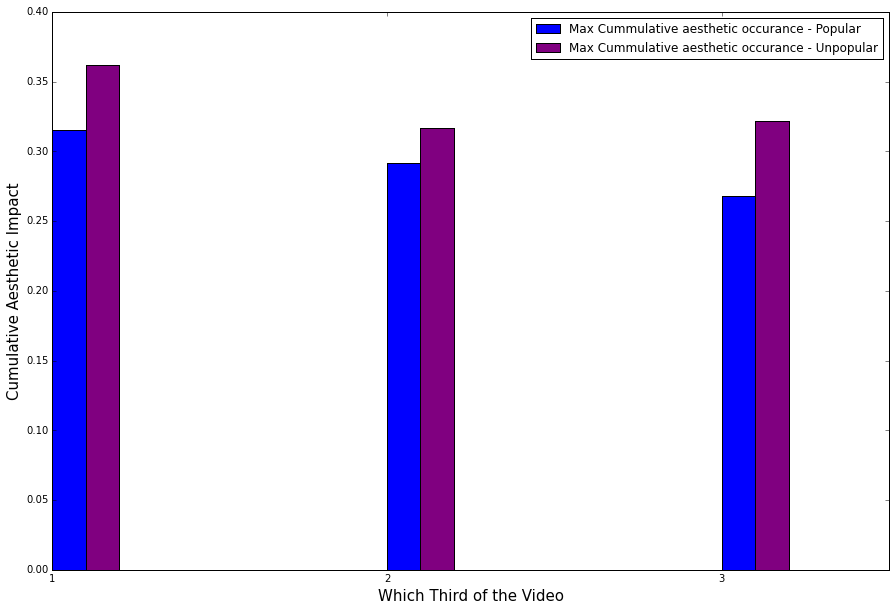
\includegraphics[width=\columnwidth]{plots/cumulativeAestheticImpact}
%\caption{\textsl{ Plot of cumulative aesthetic impact of each third of the video. For this plot the videos were sampled at one frame a second, and aesthetic features were calculated at every second. Finally the features were  }}
%\label{fig:Aesthetic_trends}
%\end{figure} 

%These two trends say something about the producer behaviour. 
%\ns{How should I close this insight? What should I draw any conclusion from this or let the classifier experiment talk about it ?} \mr{I tried something}. 
%Given that Vine engaging dynamics are influenced by the fast pace of the scrolling-based platform design, creators might want to catch the users' attention as soon as the video is appears (through scrolling) in their screen. If they are able to capture the user's glance, she will stop scrolling and start watching the video. Therefore, creators should make the initial frames  of the micro-video as ``catchy" as possible, charging them with strong emotional or aesthetic value. \mr{Should we say something about the fact that this actually works given the last results from sagar?}.

%\subsection{Quality matters, but not that much}

